\documentclass[11pt]{article}

\usepackage{amsmath}
\usepackage{amsfonts} 
\usepackage{amsthm}
\usepackage{caption}
\usepackage{enumitem} 
\usepackage{soul}
\usepackage{mathtools}
\usepackage{clrscode3e}
\usepackage{graphicx}
\usepackage{listings}
\usepackage{tikz}
\usepackage{xcolor}
\usetikzlibrary {arrows.meta,bending}
\usepackage[top=2cm,bottom=2cm,left=1.5cm,right=2cm,marginparwidth=1.75cm]{geometry}
\setlength{\parindent}{0cm}

\newcommand{\R}{\mathbb{R}}
\newcommand{\n}{\vspace{0.3cm}}

\def\rto{\color{red}{\to}\color{black}}

\def\lc{\left\lceil}   
\def\rc{\right\rceil}
\def\lf{\left\lfloor}   
\def\rf{\right\rfloor}

\newtheorem{theorem}{Theorem}

\title{\vspace{-1.0cm}\textbf{CSCI 5103 Assignment 4}}
\date{March 20, 2023}
\author{\textbf{Fletcher Gornick}\\(x500: gorni025, ID: 5579904)}

\begin{document}
\maketitle

\begin{enumerate}
  \item Consider a system consisting of \(m\) instances of a resource of some type being shared by \(n\) processes.  Prove that the system is deadlock-free if the following two conditions are satisfied:
    \begin{enumerate}[label=(\arabic*)]
      \item MaxNeed\((i) > 0\) for \(i=1,2,3,\hdots,n\), \underline{and} MaxNeed(i) is the max declared need of Process \(i\).
      \item The sum of the maximum needs of all processes is less than \((m+n)\).  (Hint: Consider proving through contradiction.)
    \end{enumerate}

    \begin{proof}
      Suppose, to the contrary, (1) and (2) hold, but the system is not deadlock-free.  This means we can come up with an assignment of resources such that some subset of processes don't reach their max need, but all \(m\) resources are used up. \n

      First notice that if there's an assignment of resources that leads to a deadlock, but at least one process actually finished, then we can come up with a different assignment such that even that process doesn't finish.  This is because if process \(i\) completes with max need \(j\), but distributing out it's resources to the remaining \(n-1\) processes leads to a deadlock, then we could instead initially assign process \(i\) no resources, and give the rest out to the other processes to cause a deadlock with all \(n\) processes. This is assuming process \(i\) has max need \(\geq 1\), which is already given in (1).\n

      So assume we've allocated our resources in a way such that NO process can finish, meaning we've used all \(m\) resources, but each process is waiting.  Letting Resources\((i)\) denote the number of resources process \(i\) currently has in this deadlock, we get the following inequality:
      \[m = \sum_{i=1}^n \text{Resources}(i) \leq \sum_{i=1}^n (\text{MaxNeed}(i)-1) = \sum_{i=1}^n \left(\text{MaxNeed}(i)\right) - n < (m+n) - n = m.\]

      But this tells us \(m < m\), which is a contradiction.  Therefore it must be the case that our system is deadlock-free, and we can conclude the above claim holds.
    \end{proof}
    

  \item Consider a system with multiple resource types which checks the safety condition using the single-resource type Banker's algorithm for each type.  Give an example of when the safety condition for each type is satisfied, but the system itself is not in a safe state.  That is, with respect to each individual resource type, the system may be in a safe state, but it would be unsafe according to the multiple-resource type Banker's algorithm.  In your example, only consider the case of \underline{two resource types}. \n

    Take the system with processes \(P_1, P_2\) and resource types \(A, B\).  There are two instances of each type in our system.  Currently, \(P_1\) has one resource of type \(A\) and none of type \(B\), \(P_2\) has none of type \(A\) and one of type \(B\).  Both need a total of two of each resource to terminate:
    \[\text{available: } (1,1), \quad P_1 \text{ needs } (1,2), \quad P_2 \text{ needs } (2,1)\]
    Clearly, this system is unsafe, but if we look at the single-resource types, we get two safe systems.  Notably, for resource \(A\), sequence order \((P_1,P_2)\) finishes, and for resource \(B\), sequence order \((P_2,P_1)\) finishes.

  \newpage
  \item \begin{enumerate}
      \item Assume that we have a paged memory, which is being used in ``real mode'' (i.e. without virtual memory).  The page table is stored in the main memory.  The memory access time is 200 nanoseconds.  This system uses a TLB, which takes 10 nanoseconds for searching.  It was found to have a hit rate of 90\%.  What is the effective memory access time \((t)\) for this system? \n

      Time to access memory on TLB hit: \(T_a = 10 + 200 = 210\) ns \\
      Time to access memory on TLB miss \(T_b = 10 + 200 + 200 = 410\) ns \\
      With hit-ratio \(H = 90\%\), we can use the equation \(t = H \cdot T_a + (1-H) \cdot T_b\):
      \[\text{effective memory access time } t = 0.9 \cdot 210 + (1-0.9) \cdot 410 = 230 \text{ nsec.}\]

      \item Now suppose that this system with the TLB data given above is a demand paged virtual memory system.  It takes 5 milliseconds to service a page-fault if an empty frame is available or if the replaced page is not modified, and 10 milliseconds if the replaced page is modified (i.e. dirty).  Assume that 40\% of the time an empty frame is available or the page to be replaced is not modified. What is the maximum acceptable page-fault rate for an effective access time of no more than 250 nanoseconds? \n

        Note that 5 ms = 5000000 ns, and 10 ms = 10000000 ns.  Now let's first calculate the average amount of time it takes to recover from a page-fault (call this value \(f\)):
        \begin{align*}
          f &= P(\text{clean/empty frame}) \cdot (\text{clean service time}) + P(\text{dirty page}) \cdot (\text{dirty service time}) \\
            &= 0.4 \cdot 5000000 + 0.6 \cdot 10000000 \\
            &= 8000000 \text{ ns (8 ms)}.
        \end{align*}
        Now we have the following equation for effective memory access time \(t\) dependent on memory access time \(a\), probability of page-fault \(p\), and page-fault service time \(f\):
        \[t = (1-p) \cdot a + p \cdot f \implies p = \frac{t-a}{f-a}\]
        Plugging in \(t = 250\), \(a = 200\), and \(f = 8000000\), we get:
        \[\text{page-fault rate } p = \frac{t-a}{f-a} = \frac{250-200}{8000000-200} = 6.25 \times 10^{-6}.\]
        So we can only have page-faults \(6.25 \times 10^{-4}\) percent of the time max in order to guaruntee an effective memory access time of 250 nsec.  In other words, we can have one page-fault every 159996 accesses.
    \end{enumerate} \n

  \item \begin{enumerate}
      \item Consider a page reference string: \((2, 3, 5, 3, 5, 1, 2)\). \\
      Given three page-frames, how many page-faults will happen with each of the following page-replacement algorithms: LRU and FIFO? \\
      Assume that initially these three frames are empty. \n

      In this case, the algoritm for LRU and FIFO are actually the exact same
      \[\begin{pmatrix} - \\ - \\ - \end{pmatrix} \rto \begin{pmatrix} 2 \\ - \\ - \end{pmatrix} \rto \begin{pmatrix} 2 \\ 3 \\ - \end{pmatrix} \rto \begin{pmatrix} 2 \\ 3 \\ 5 \end{pmatrix} \to \begin{pmatrix} 2 \\ 3 \\ 5 \end{pmatrix} \to \begin{pmatrix} 2 \\ 3 \\ 5 \end{pmatrix} \rto \begin{pmatrix} 1 \\ 3 \\ 5 \end{pmatrix} \rto \begin{pmatrix} 1 \\ 2 \\ 5 \end{pmatrix}, \;\; \text{so 5 page-faults.}\]

      \item Extend the reference string in part (a) above with a small number of additional page references to yield an example in which LRU is better than FIFO for the case of three page-frames. \n\\
        \((2, 3, 5, 3, 5, 1, 2, 5, 4, 5)\) yields 6 page-faults for LRU and 7 page-faults for FIFO. \n

      \item Now, extend this string in part (a) above with a different sequence of page references to yield an example in which FIFO is better than LRU for the case of three page-frames. \n\\
        \((2, 3, 5, 3, 5, 1, 2, 5, 4, 1)\) yields 7 page-faults for LRU and 6 page-faults for FIFO.
    \end{enumerate} \n

  \item Consider a system using the WSclock scheme for working-set based virtual memory management.  Suppose that the current virtual time is 2000.  This system had 8 page frames.  Figure below shows the position of the clock hand, and the values of the last-time-of-use and the R bit for each frame.
    \begin{center}
      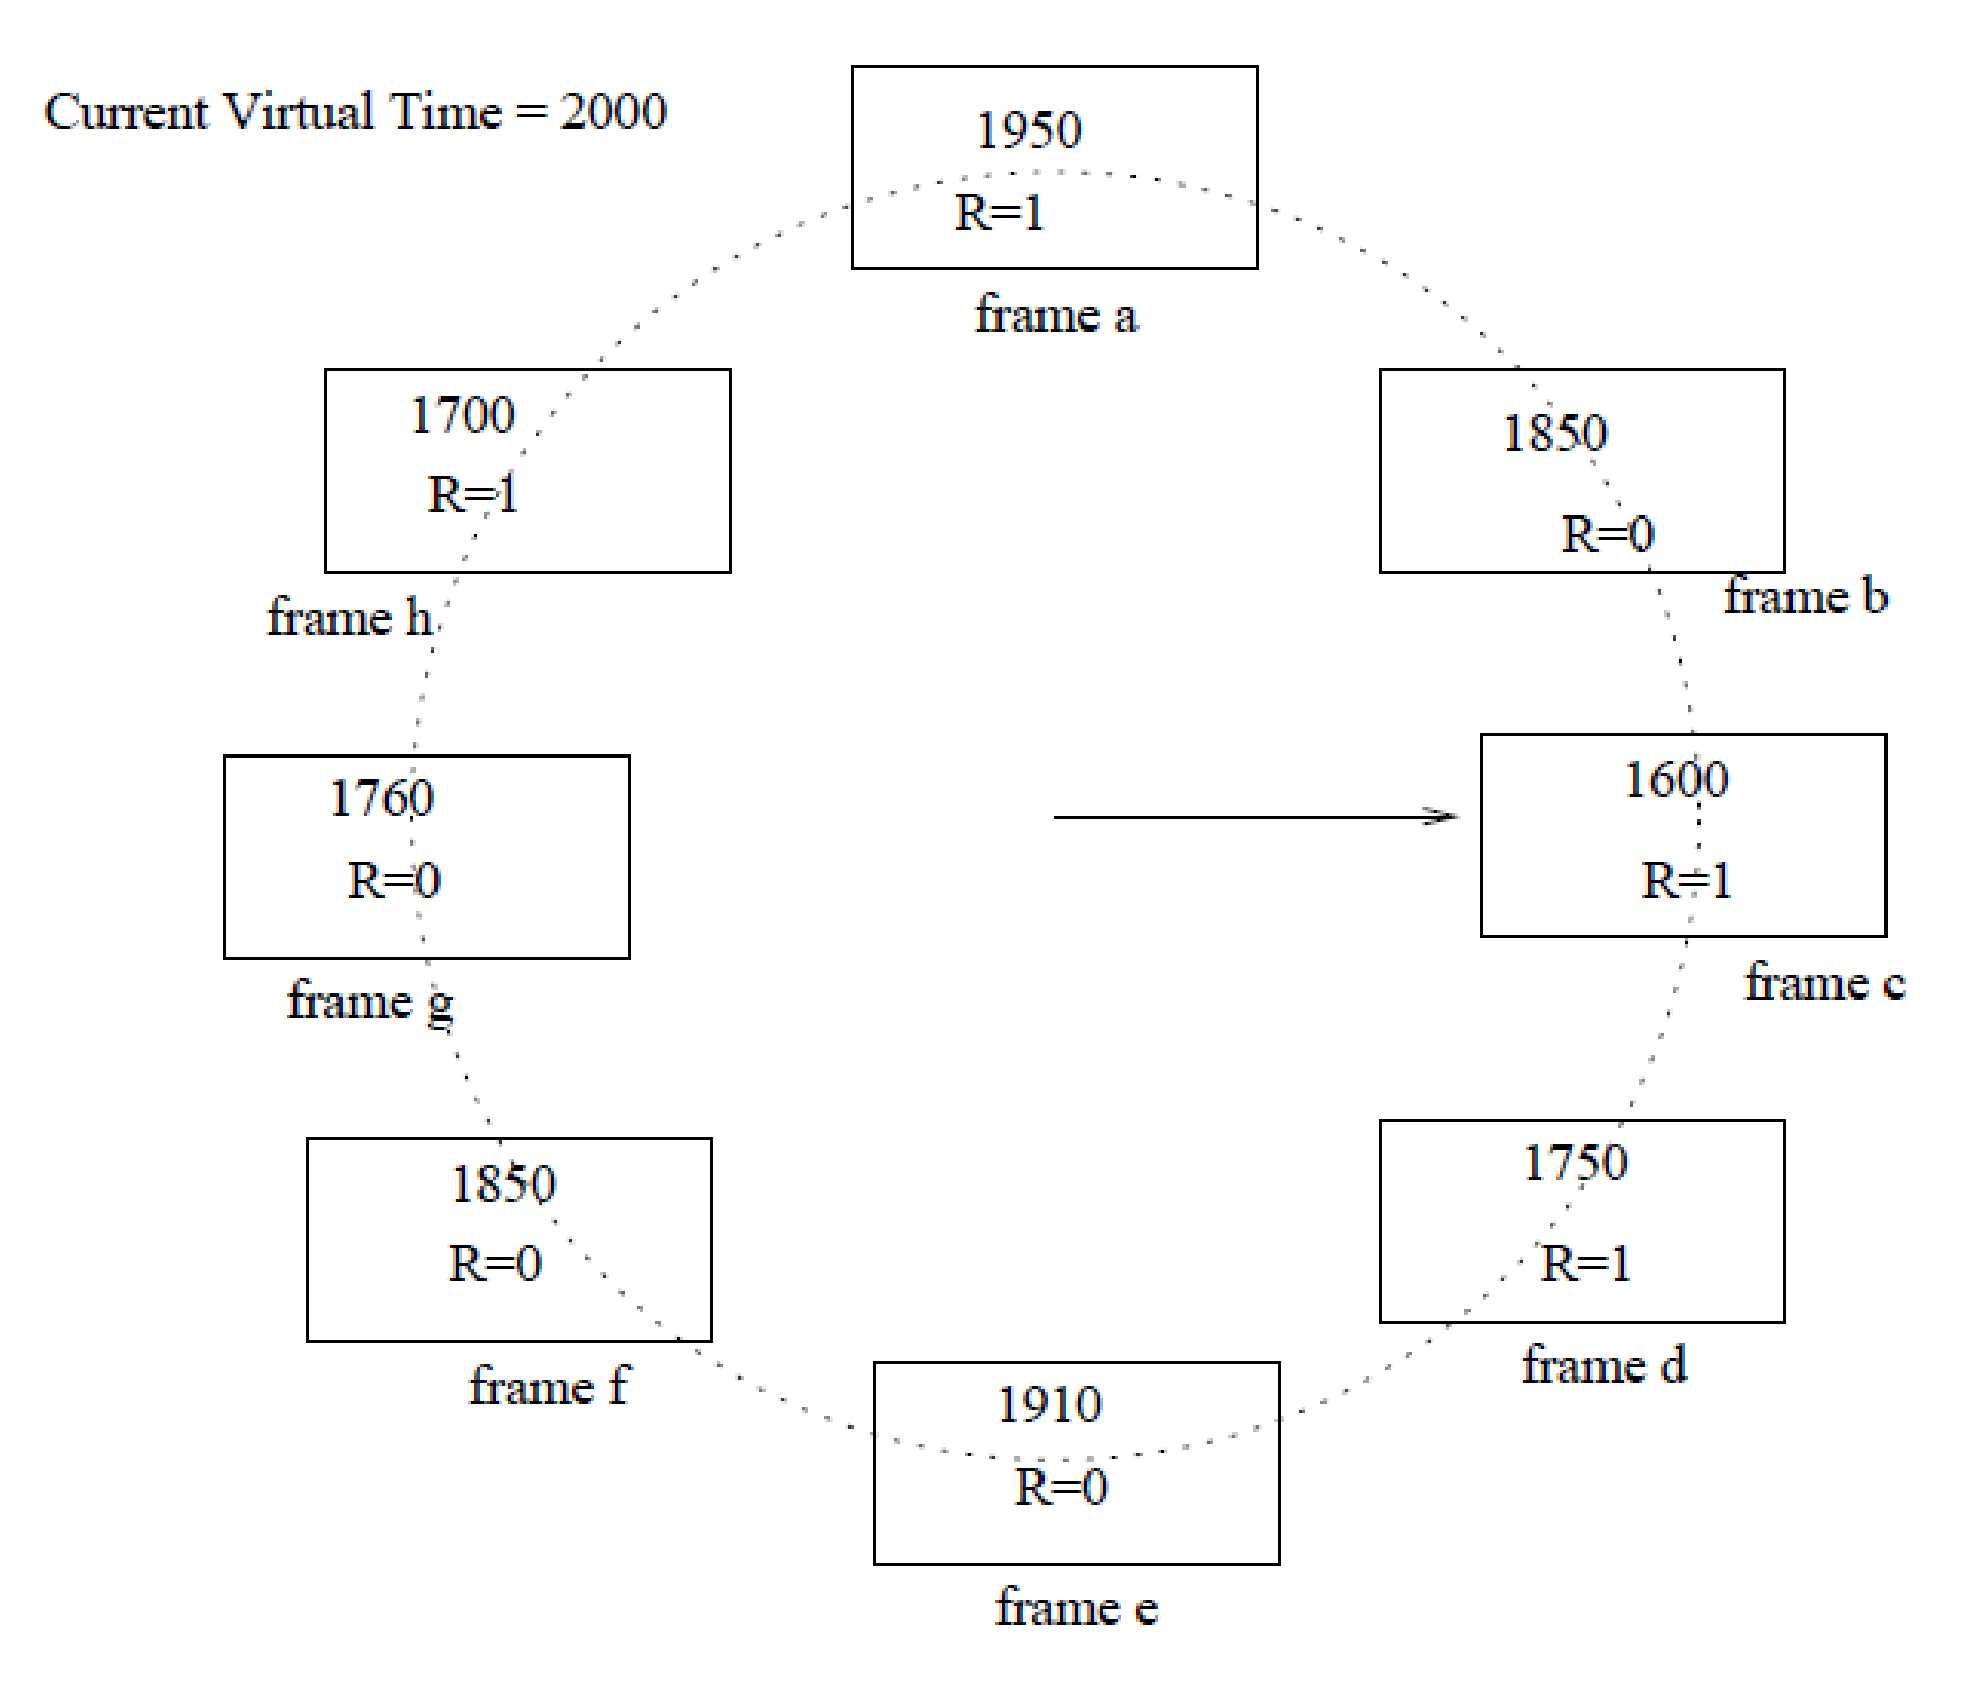
\includegraphics[width=0.75\textwidth]{5.png}
    \end{center}
    \begin{enumerate}
      \item Suppose that the periodic clock interrupt comes virtual time 2000.  Show the new contents of all the frame-list records. \n

        To update our frames, we simply go to each frame and:
        \begin{enumerate}
          \item If it's reference bit is 0: skip
          \item If it's reference bit is 1: switch it to 0 and change last-time-of-use to 2000
        \end{enumerate}
        This gives us the following frame-list records:
        \begin{center}
          \begin{tabular}[c]{|l|c|c|c|c|c|c|c|c|}
            \hline
            frame & a & b & c & d & e & f & g & h \\
            \hline
            last-time-of-use & 2000 & 1850 & 2000 & 2000 & 1910 & 1850 & 1760 & 2000 \\
            \hline
            reference bit & 0 & 0 & 0 & 0 & 0 & 0 & 0 & 0 \\
            \hline
          \end{tabular} \n
        \end{center}
        
      \item Now suppose that instead of the clock interrupt a page-fault occurs at virtual time 2000.  For each of the two values of \(\tau\) \textbf{equal to 100 and 200}:
        \begin{enumerate}
          \item Indicate the frame whose page is replaced. \n
            \begin{enumerate}
              \item[(\(\tau = 100\))] The frame that get's removed is the first frame (starting from frame c), with reference bit 0, whose last time of use is less than \(2000 - 100 = 1900\).

                Frame c: \(R=1\), frame d: \(R=1\), frame e: \(LR(e) = 1910 \geq 1900\), frame f: perfect!  So the frame that's replaced is \textbf{f}. \n

              \item[(\(\tau = 200\))] The frame that get's removed is the first frame (starting from frame c), with reference bit 0, whose last time of use is less than \(2000 - 100 = 1800\).

                Frame c: \(R=1\), frame d: \(R=1\), frame e: \(LR(e) = 1910 \geq 1800\), frame f: \(LR(f) \geq 1800\), frame g: perfect!  So the frame that's replaced is \textbf{g}.
            \end{enumerate} \n

          \item Show the new contents of the frame-list. \n
            \begin{enumerate}
              \item[(\(\tau = 100\))] 
                \begin{center}
                  \begin{tabular}[c]{|l|c|c|c|c|c|c|c|c|}
                    \hline
                    frame & a & b & c & d & e & f & g & h \\
                    \hline
                    last-time-of-use & 1950 & 1850 & 2000 & 2000 & 1910 & 2000 & 1760 & 1700 \\
                    \hline
                    reference bit & 1 & 0 & 0 & 0 & 0 & 1 & 0 & 1 \\
                    \hline
                  \end{tabular}
                \end{center} \n

              \item[(\(\tau = 200\))]
                \begin{center}
                  \begin{tabular}[c]{|l|c|c|c|c|c|c|c|c|}
                    \hline
                    frame & a & b & c & d & e & f & g & h \\
                    \hline
                    last-time-of-use & 1950 & 1850 & 2000 & 2000 & 1910 & 1850 & 2000 & 1700 \\
                    \hline
                    reference bit & 1 & 0 & 0 & 0 & 0 & 0 & 1 & 1 \\
                    \hline
                  \end{tabular} \n
                \end{center}
            \end{enumerate} \n

          \item Determine which logical pages (and thus the corresponding frames storing those pages) will be candidates for removal from the working set. \n

            \begin{enumerate}
              \item[(\(\tau = 100\))] For \(\tau = 100\), frames b,f, and g are all candidates for removal, as they're all old enough and not being referenced. \n

              \item[(\(\tau = 200\))] For \(\tau = 200\), frames g is the only candidate for removal, as it's the only frame with 0 reference bit that was used before virtual time 1800.
            \end{enumerate}
        \end{enumerate}
    \end{enumerate} \n
    
  \item Suppose that the page-reference string of a process contains repetitions of long sequences of page references in the range 0 through 511, followed occasionally by a random reference to a page number in the range 512 to 1023.  For example, the sequence: \(0, 1, \hdots, 510, 511, 600, 0, 1, \hdots, 510, 511, 700, 0, 1, \hdots\) consists of the repetitions of the sequence \(0, 1, \hdots, 510, 511\) followed by a random reference to pages such as 600 and 700. Assume that this sequence repeats \(N\) times. \n\\
    \textbf{NOTE:} for both of these parts, I assume the first iteration page-faults 100\% of the time, because I'm under the assumption that our buffer is empty at the start.

    \begin{enumerate}
      \item If 511 frames are given to this process, how many page-faults would occur using the LRU replacement policy when this sequence repeats for \(N\) times?  Answer the this question for the FIFO replacement policy. \n

        First, note that since these page numbers come in the same order, the least recently used page is also the oldest one to be thrown into the lookup table, so LRU and FIFO will act the same. \n

        The first 511 pages will page-fault, as our table is empty, then when we get to 511, we miss again and replace 0.  Next, we hit our first random reference page, this page-faults and replaces 1. \n

        On the next iteration, for the sequence of page numbers \(0 \leq i \leq 509\), we page-fault every time, and our victim is frame \((i+2)\).  It's not hard to see that these replacement policies lead to a page-fault on every new frame. \n

        Repeating \(N\) times, we get that LRU and FIFO policies result in \(513N\) page-faults. \n

      \item With 511 frames allocated to this process, describe a page replacement scheme that would perform much better than LRU or FIFO.  Give the number of page-faults for your proposed replacement scheme when this sequence repeats for \(N\) times?  You may assume that the replacement scheme has knowledge of the access pattern in the page reference string, as described above. \n

        In this case, the better replacement policy would be \textbf{Highest Frame Number}. \n

        Just like above, on our first iteration there will be 513 page faults (as our buffer is initially empty), but now our buffer will contain page numbers (\(0,1,\hdots,508,509,600\)). \n

        On our next iteration, we won't have any page faults until we get to 510.  At this point we replace 600, then we get 511 which faults and replaces 510.  Finally, we get some \(n\) between 512 and 1023 that faults and replaces 511. \n

        This iteration results in page numbers (\(0,1,\hdots,508,509,n\)) in our buffer, and only page-faults 3 times, so any subsequent iteration using this replacement policy will only fault 3 times as well.  This gives us the following equation for number of page-faults depending on number of times the sequence repeats \(N\) (assume \(N \geq 1\)):
        \[\text{number of page-faults } P = 513 + 3 \cdot (N-1).\]

        If instead, we were to assume that our buffer initially starts with page numbers \((0,1,\hdots,508,509)\) already in it, then it would result in only \(3N\) page-faults via the \textit{Highest Frame Number} replacement policy.
    \end{enumerate} \n

  \item Please read Chapters 1 and 2 from the book O’Reilly book ``Linux Device Drivers'', and answer the following question: \\
    What is the purpose of the following kernel functions?
    \begin{enumerate}
      \item insmod \n\\
        The linux kernel offers a limited set of features, and it has the ability to add-to / delete-from that set of features without ever needing to shut down.

        The code that's added or removed from our set of features is called a \textit{module}.  Modules are made up of object code but not linked into a runnable executable yet.

        The function \textit{insmod} is used to dynamically link the object code of a specified module to the running kernel.  Also worth noting, is the function \textit{rmmod}, which just unlinks a specified module from our running kernel. \n

      \item lsmod \n\\
        lsmod just lists the currently loaded kernel modules.  If you have a c progran compiled to a kernel module (file ending in \textit{.ko}) that's not currently listed with lsmod, then you can use the following command to add it, so on a subseqent call to ``lsmod'' it will be listed:\begin{verbatim}
                          sudo insmod <filename>.ko
        \end{verbatim} 
      \item module\_init \n\\
        module\_init is the function that's invoked immediatly after a call to insmod.  It defines any of the setup to be done for future calls of the module's functions.  Modules don't actively do anything, they're event-driven, so module\_init just sets up the modules resources, and future calls to a module function are what actually trigger functionality. \n

      \item module\_exit \n\\
        This function is invoked just before the module is unloaded from the running kernel, this method is invoked after a call to rmmod.  The job of module\_exit is to deallocate any resources that module\_init initialized for our module.  It's important that module\_exit undoes everything, as if it doesn't, then those non-deleted resources will remain in the system until restarted.
    \end{enumerate}
\end{enumerate}
\end{document}
